\documentclass{article}

\usepackage[english]{babel}
\usepackage[a4paper,top=2cm,bottom=2cm,left=3cm,right=3cm,marginparwidth=1.75cm]{geometry}
\usepackage[backend=biber, sorting=nyt, style=authoryear-ibid]{biblatex}
%\bibliographystyle{agsm}
%\let\cite\textcite

\usepackage{amsmath}
\usepackage{csquotes}
\usepackage{graphicx}
\graphicspath{ {figures/} }
\usepackage[colorlinks=true, allcolors=blue]{hyperref}
\usepackage{parskip}
\usepackage{multirow}
\usepackage{fontspec}
\usepackage{fontawesome5}
%\newcommand{\faWindows}{\FA\symbol{"F17A}}
%\newcommand{\faLinux}{\FA\symbol{"F17C}}
%\newcommand{\faApple}{\FA\symbol{"F179}}

%\bibliography{references}
\addbibresource{references.bib}

\title{Mockingjay Assignment Literature Review}
\author{Stuart Kingham}

\begin{document}
\maketitle

\begin{abstract}
Literature review.
\end{abstract}

\tableofcontents

\section{Intro}

Cite using:
\begin{enumerate}
\item \textbf{citetitle\{Smith:2012jd\}}: \citetitle{Smith:2024jd}
\item \textbf{parencite\{Smith:2012qr\}}: A citation command in parentheses: \parencite{Smith:2023qr}.
\item \textbf{textcite\{Smith:2024jd\}}: For use in the flow of text: As \textcite{Smith:2024jd} said \dots
\item \textbf{autocite\{Peixoto:2023\}}: A citation command which automatically switches style depending on
  location and the option setting in the package declaration (see line 12 in the LaTeX source code). In this
  case, it produces a citation in parentheses: \autocite{Peixoto:2023}.
\end{enumerate}

\subsection{Host-based code injection attack (HBCIA) techniques}

Process injection refers to different methods employed to deliver malicious code into the memory space of a
running process.  The technique enables attackers to hide the injected code \textit{how?} and evade detection.

In a Windows \faWindows \space environment, attackers rely on a combination of Windows APIs to effect the injection
process \textit{what are these? Are they all the same, can they be categorised?}.

Security solutions are aware of these techniques and have measures to detect and block the injection process based
on the patterns of executed calls in the OS during the infection.  A promenant adveserial challenge by \textbf{EDR}
systems is to set hooks on the NT system API calls within the memory space of every launched process on protected
systems.  These hooks intercept and capture the calling parameters to Windows APIs to identify potentially malicious actions.

The security team at Security Joes looked to ``discover alternative methods to dynamically execute code within
the memory space of Windows processes, without relying on monitored Windows APIs.''  Their process involved
finding trusted Windows libraries that have sections \textit{what is a section and why is it important to this?}
with default protections set as Read-Write-eXecute (RWX).  Code was demonstrated that injected code into various
processes, eliminating the need to execute several Windows API calls usually monitored by security solutions.
As the attack does not directly invoke Windows API calls usually associated with process injection techniques.

Their starting point is a HBCIA \textit{check assumption that the attack is a hollowing out, hence destructive to the host proces - must be better term than host process. If it is destructive, then cannot by HBCI/RBCI; must be an attack} identifying a process with a section that can be attacked.  They then show how they can construct a RBCIA.

\subsubsection{\citetitle{Barabosch:2014}}
\textcite{Barabosch:2014}  Formalises HBCIA\/RBCIA and key components, attack algorithm taxonomy, prevalence estimation.
\iffalse
\fi
Differentiate between HBCI and HBCIA, HBCI \& RBCI.

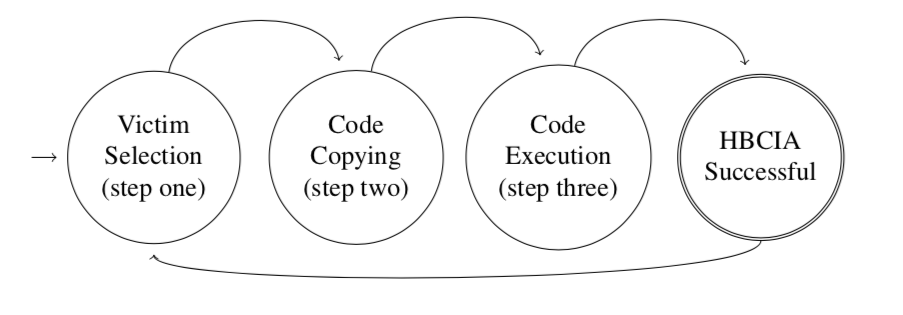
\includegraphics[scale=0.4]{hbcia_3step_algo.png}

\subsubsection{\citetitle{Ghizzoni:2004}}
\textcite{Ghizzoni:2004} MS Patent.


\subsubsection{\citetitle{Jang:2007}}
\textcite{Jang:2007}

Looking at memory paging of compromised processes: \citetitle{Pek:2016}, \autocite{Pek:2016}.


Need to introduct reinforcement techniques used by endpoint security:

HBCI:

\subsection{EDR}

Review EDR capabilities.  To counter process injection attacts EDR systems can:

\begin{itemize}
\item Static Monitoring of specific DLLs or System Calls: The first level of protection against process injection attack techiques is
  scan processes \ldots
\item Behavioural Analysis: User and entity behaviour analytics (UEBA) are being introduced into XDR tools \ldots
\item Anomaly detection: \autocite{Pek:2016} \ldots
\item Machine Learning techniques: \autocite{Wang:2022}
\end{itemize}

\subsubsection{\citetitle{Wang:2022}}
\textcite{Wang:2022}

\subsection{Mockingjay}

The Mockingjay  attack targets trusted and legitimate processes runing on a sytem.  

\subsubsection{\citetitle{Peixoto:2023}}
\textcite{Peixoto:2023}

\textbf{Why is this technique important?}: It's a new potential security vulnerability. It is a process injection
technique utilised byattackers to deceive robust security products in a corporate environment, such as ``EDRS'' and \textbf{XDRS}.

Process is designed to bypass security controls to gain unauthorised access.


\section{Background Literature Review}

% Section 2 is a literature review of HBCI methods and endpoint security that is typically relied upon to prevent these types of attack.  We will then look at methods a identifying these attacks and look at the likelihood of Endpoint Security products of identifying the attack.

\subsection{Endpoint Security: EDR}

\subsubsection{\citetitle{Hayes:2023}}
\textcite{Hayes:2023}


\subsection{Code Injection Methods}

\subsubsection{\citetitle{Mitre:2017}}
\textcite{Mitre:2017}

\begin{itemize}
\item T1055.001	Dynamic-link Library Injection
\item T1055.002	Portable Executable Injection
\item T1055.003	Thread Execution Hijacking
\item T1055.004	Asynchronous Procedure Call
\item T1055.005	Thread Local Storage
\item T1055.008	Ptrace System Calls
\item T1055.009	Proc Memory
\item T1055.011	Extra Window Memory Injection
\item T1055.012	Process Hollowing
\item T1055.013	Process Doppelgänging
\item T1055.014	VDSO Hijacking
\item T1055.015	ListPlanting
\end{itemize}


\begin{table}[h!]
\centering
\begin{tabular}{ |p{1.2cm}||p{2cm}|p{11.5cm}|  }
  \hline
  \multicolumn{3}{|c|}{PI Mitigation List} \\
  \hline
  ID	& Mitigation & Description \\
  \hline
  M1040	& Behavior Prevention on Endpoint &	Some endpoint security solutions can be configured to block some types of
                                            process injection based on common sequences of behavior that occur during the
                                            injection process. For example, on Windows 10, Attack Surface Reduction (ASR)
                                            rules may prevent Office applications from code injection. [78] \\
  \hline
  M1026 & Privileged Account Management	& Utilize Yama (ex: /proc/sys/kernel/yama/ptrace\_scope) to mitigate ptrace based
                                          process injection by restricting the use of ptrace to privileged users only. Other
                                          mitigation controls involve the deployment of security kernel modules that provide
                                          advanced access control and process restrictions such as SELinux, grsecurity,
                                          and AppArmor. \\
  \hline
\end{tabular}
\label{table: Mitigations}
\end{table}

\begin{table}[h!]
\centering
\begin{tabular}{ |p{1.2cm}||p{2cm}|p{3cm}|p{8cm}|  }
  \hline
  \multicolumn{4}{|c|}{PI Detection List} \\
  \hline
  ID	& Data Source & Data Component & Detects \\
  \hline
   & & & \\
  DS0022 & File & File Metadata & Monitor for contextual data about a file, which may include information such as name,
                                  the content (ex: signature, headers, or data/media), user/ower, permissions, etc. \\
        & & File Modification & Monitor for changes made to files that may inject code into processes in order to evade
                                process-based defenses as well as possibly elevate privileges. \\
  \hline
  DS0011 & Module & Module Load & Monitor DLL/PE file events, specifically creation of these binary files as well as
                                  the loading of DLLs into processes. Look for DLLs that are not recognized or not
                                  normally loaded into a process. \\
  \hline
  DS0009 & Process & OS API Execution & Monitoring Windows API calls indicative of the various types of code injection
                                        may generate a significant amount of data and may not be directly useful for
                                        defense unless collected under specific circumstances for known bad sequences
                                        of calls, since benign use of API functions may be common and difficult to
                                        distinguish from malicious behavior. Windows API calls such as CreateRemoteThread,
                                        SuspendThread/SetThreadContext/ResumeThread, QueueUserAPC/NtQueueApcThread, and
                                        those that can be used to modify memory within another process, such as
                                        VirtualAllocEx/WriteProcessMemory, may be used for this technique.[79] Monitoring
                                        for Linux specific calls such as the ptrace system call should not generate large
                                        amounts of data due to their specialized nature, and can be a very effective
                                        method to detect some of the common process injection methods.[80] [81] [82] [83] \\
        & & Process Access & Monitor for processes being viewed that may inject code into processes in order to
                             evade process-based defenses as well as possibly elevate privileges. \\
        & & Process Metadata & Monitor for process memory inconsistencies, such as checking memory ranges against a
                               known copy of the legitimate module.[84] \\
        & & Process Modification & Monitor for changes made to processes that may inject code into processes in order
                                   to evade process-based defenses as well as possibly elevate privileges. \\
  \hline
\end{tabular}
\label{table: Detection}
\end{table}

\pagebreak

\subsubsection{\citetitle{Hosseini:2017}}
\textcite{Hosseini:2017}

\begin{table}[h!]
\centering
\begin{tabular}{ |p{3.5cm}||p{1.2cm}|p{10cm}|  }
  \hline
  \multicolumn{3}{|c|}{Ten process injection techniques} \\
  \hline
  Name	& ID & Description \\
  \hline
  Classic Dll Injection Via Createremotethread And Load Library
        & T1055 .001
             & The malware writes the path to its malicious dynamic-link
               library (DLL) in the virtual address space of another process,
               and ensures the remote process loads it by creating a remote thread in the target process. \\
  \hline
  Portable Executable (PE) Injection
        & T1055 .002
             & Copy malicious code into an existing open process and cause it to execute (either via a
               small shellcode, or by calling CreateRemoteThread). The malware does not have to drop a
               malicious DLL on the disk; still allocates memory in a host process (e.g. VirtualAllocEx),
               but writes its malicious code by calling WriteProcessMemory. \\
  \hline
  Process Hollowing (A.K.A Process Replacement and Runpe)
        &
             & malware unmaps (hollows out) the legitimate code from memory of the target process, and
               overwrites the memory space of the target process (e.g., svchost.exe) with a malicious executable.\\
  \hline
  Thread Execution Hijacking (A.K.A Suspend Inject and Resume (SIR)
        & T1055 .003
             & After getting a handle to the target thread, the malware puts the thread into suspended mode by
               calling SuspendThread to perform its injection. The malware calls VirtualAllocEx and
               WriteProcessMemory to allocate memory and perform the code injection. Targeting an existing thread
               of a process, during analysis you will probably see calls to CreateToolhelp32Snapshot and
               Thread32First followed by OpenThread. \\
  \hline
  Hook Injection via Setwindowshookex
        &
             & Malicious DLL loaded upon an event getting triggered in a specific thread. This is usually
               done by calling SetWindowsHookEx to install a hook. \\
  \hline
  Injection and Persistence via Registry Modification (E.G. Appinit\_DLLS, AppCertDLLs, IFEO)
        &
             & Appinit\_DLL, AppCertDlls, and IFEO (Image File Execution Options) are all registry keys that
               malware uses for both injection and persistence. \\
  \hline
  APC Injection And Atombombing
        & T1055 .004
             & Use APC to force another thread to execute their custom code by attaching it to the APC
               Queue of the target thread. \\
  \hline
  Extra Window Memory Injection (EWMI) via Setwindowlong
        &
             & Injecting into Explorer tray window’s extra window memory, and has been used a few times
               among malware families such as Gapz and PowerLoader. There is not much room in EWM, so the
               malware writes code into a shared section of explorer.exe, and uses SetWindowLong and
               SendNotifyMessage to have a function pointer to point to the shellcode, and then execute it. \\
  \hline
  Injection Using Shims
        &
             & Shims allow developers to apply fixes to their programs without the need of rewriting code.
               Malware can take advantage of shims to target an executable for both persistence and injection.
               Windows runs the Shim Engine when it loads a binary to check for shimming databases in order
              to apply the appropriate fixes. \\
  \hline
  At Hooking and Inline Hooking (A.K.A Userland Rootkits)
        &
            & Malware changes the import address table. When a legitimate application calls an API located
              in a DLL, the replaced function is executed instead of the original one. \\
  \iffalse
\fi
  \hline
\end{tabular}
\label{table: ProcessInjectionTechniques}
\end{table}

\pagebreak

\href{https://learn.microsoft.com/en-gb/windows/win32/sync/asynchronous-procedure-calls}{MS Asynchronous Procedure Calls}

\href{https://learn.microsoft.com/en-gb/windows/win32/winmsg/about-hooks}{Microsoft Win32 Hooks Overview: hook types and example uses}

\subsection{Deploying Payload into Windows Memory Space}

\subsubsection{\citetitle{Zhan:2018}}
\textcite{Zhan:2018}


\subsubsection{\citetitle{Dequeker:2023}}
\textcite{Dequeker:2023}


\subsubsection{\citetitle{S12h4ck:2023a}}
\textcite{S12h4ck:2023a}

\href{https://github.com/elddy/Windows-NTAPI-Injector}{GitHub.com Windows-NTAPI-Injector}

\href{https://gist.github.com/WKL-Sec/96e17188e4c159c2cdf7ff2c111130cc#file-local-c}{GitHub.com Injector examples in C}

\subsubsection{\citetitle{S12h4ck:2023b}}
\textcite{S12h4ck:2023b}

\href{https://www.unknowncheats.me/forum/anti-cheat-bypass/286274-internal-detection-vectors-bypass.html}{internal detection vectors bypass}


% Section 3 an investigation into the Mockingjay attack and against a recently published paper ``Procguard'' \cite:{Wang:2022} and asks weather this attack method would lickly be caught.
\section{Mockingjay}

% Section 4 is an implementation of the attack and will look at manually identifying an infected process and generating artifacts that could be used in automating the process.
\section{Attack Imlementation}

\section{Figures}

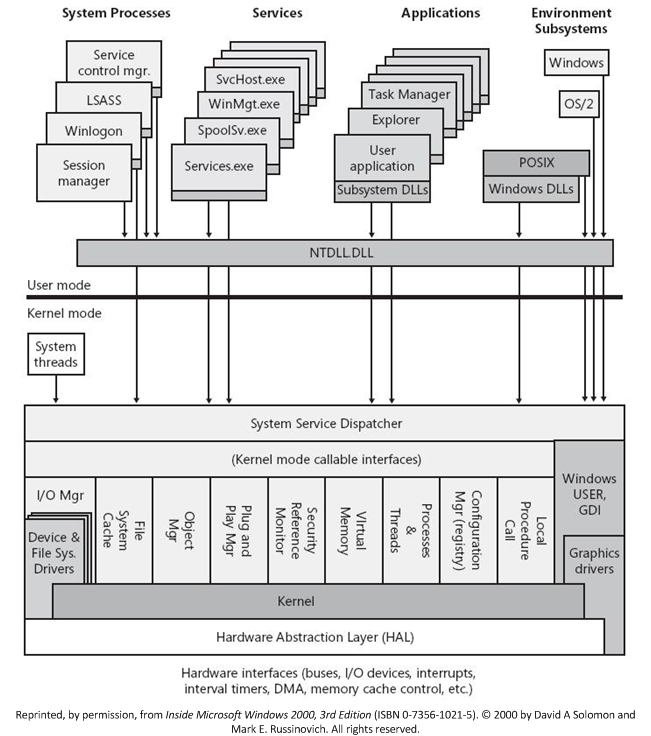
\includegraphics[scale=0.4]{ms_hardware_interfaces.png}

\printbibliography

\end{document}

%%% Local Variables:
%%% mode: latex
%%% TeX-master: t
%%% End: